\subsection{Отладка программного обеспечения}

Для отладки написанной программы использовался физический субмодуль экрана. Так как устройство можно использовать с разными моделями экрана, на плате распаян универсальный разъем, который содержит все возможные контакты матрицы. С помощью переходного шлейфа, который с одной стороны содержит разъем устройства, а с другой -- разъем матрицы, был подключен тестовый фрагмент экрана. 

Хоть и использование экрана было смелым шагом, однако отладка первых запусков была произведена при помощи логического анализатора, который упростил нахождение дефектов к программном коде.

\begin{figure}[ht]
    \centering
    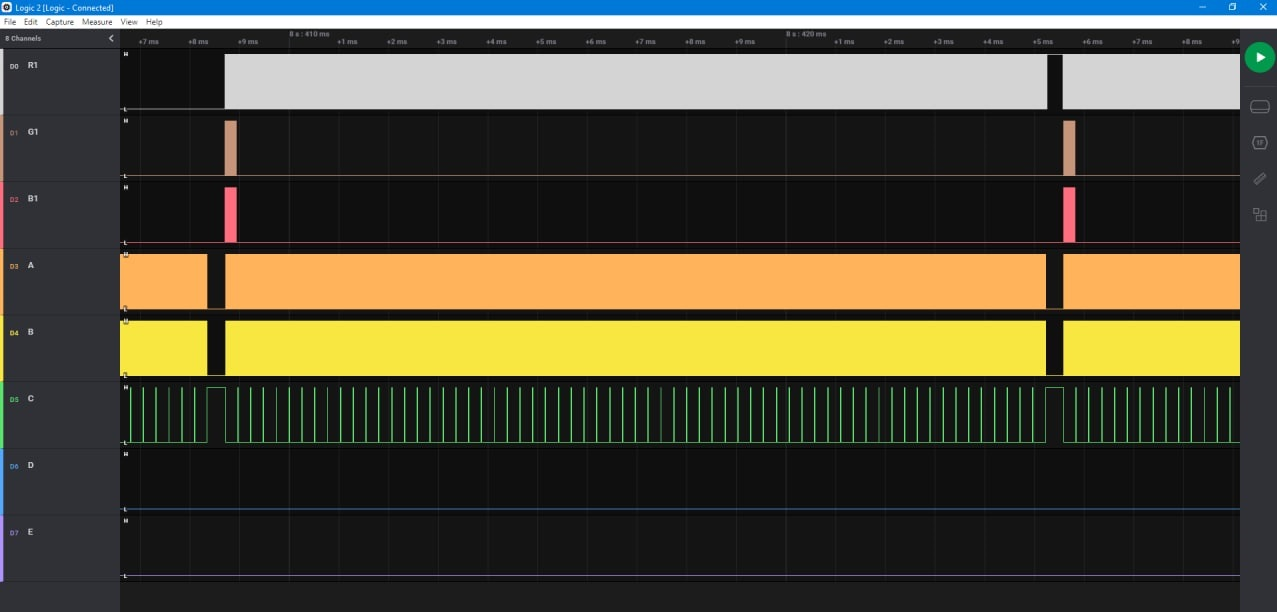
\includegraphics[width=0.8\linewidth]{\commonSecPathPrefix/sec_6/content/analizer2.jpg}
    \caption{Отладка логическим анализатором}
\end{figure}

Отладку так же упростила возможность использования точек остановки во время выполнения программы на STM32. В среде разработки \textit{STM32CubeIDE} предусмотрена возможность просмотра состояния переменных, стека вызовов, а так же состояния регистров.

\begin{figure}[ht]
    \centering
    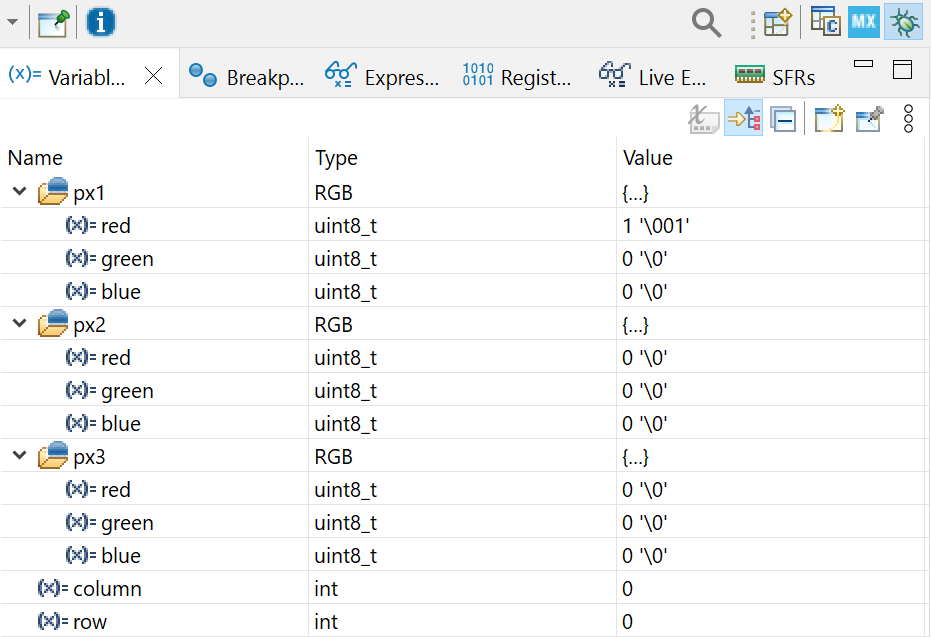
\includegraphics[width=0.6\linewidth]{\commonSecPathPrefix/sec_6/content/debug_vars.png}
    \caption{Окно состояния переменных}
\end{figure}

После проведения отладки, получилось вывести на матрицу произвольный тестовый паттрен, который облегчает поиск нерабочих светодиодов на экране. На фотографии можно наблюдать фрагмент модуля, матрицу, а так же \textbf{шлейф, которым подключается матрица к эмулятору}.

\begin{figure}[ht]
    \centering
    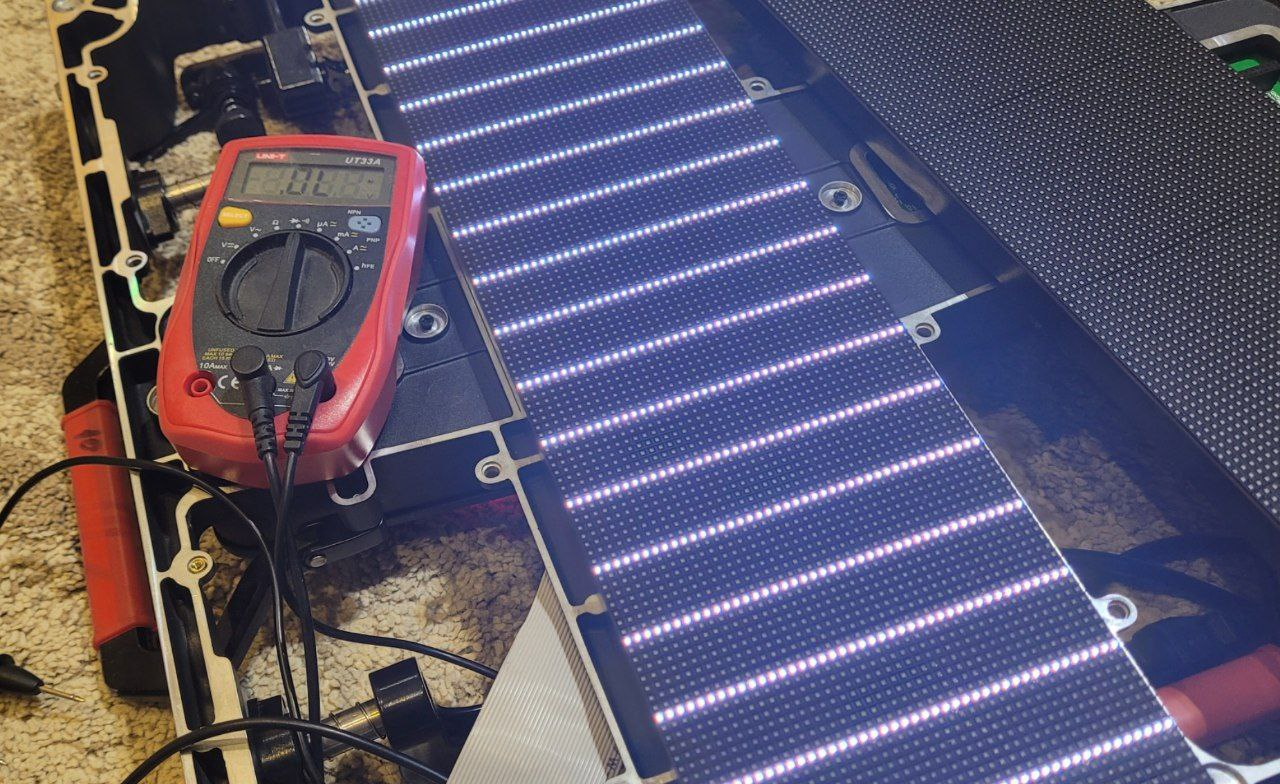
\includegraphics[width=0.9\linewidth]{\commonSecPathPrefix/sec_6/content/led_working.jpg}
    \caption{Подключенный к матрице эмулятор}
\end{figure}